%File: neurastem.tex
%NeuralStem --- course project proposal (AAAI 2026 format)

\documentclass[letterpaper]{article} % DO NOT CHANGE THIS
\usepackage{aaai2026}  % DO NOT CHANGE THIS
\usepackage{times}  % DO NOT CHANGE THIS
\usepackage{helvet}  % DO NOT CHANGE THIS
\usepackage{courier}  % DO NOT CHANGE THIS
\usepackage[hyphens]{url}  % DO NOT CHANGE THIS
\usepackage{graphicx} % DO NOT CHANGE THIS
\urlstyle{rm} % DO NOT CHANGE THIS
\def\UrlFont{\rm}  % DO NOT CHANGE THIS
\usepackage{natbib}  % DO NOT CHANGE THIS AND DO NOT ADD ANY OPTIONS TO IT
\usepackage{caption} % DO NOT CHANGE THIS AND DO NOT ADD ANY OPTIONS TO IT
\frenchspacing  % DO NOT CHANGE THIS
\setlength{\pdfpagewidth}{8.5in}  % DO NOT CHANGE THIS
\setlength{\pdfpageheight}{11in}  % DO NOT CHANGE THIS

\usepackage{array}
\usepackage{amssymb}
\usepackage{tikz}
\usetikzlibrary{arrows.meta,positioning,fit,backgrounds}

% Line-breaking policy (affects hyphenation only; page geometry, margins and
% fonts are untouched, as the template rules require).
% Prose keeps default two-column hyphenation, which gives the most even
% spacing. Table cells suppress it: a word broken across lines inside a
% narrow column reads as a typesetting error, whereas in a justified
% paragraph it is unremarkable.
% Applied inside table groups only; values are restored when the group ends.
\newcommand{\nohyph}{\hyphenpenalty=10000 \exhyphenpenalty=10000 \tolerance=10000 \emergencystretch=3em}

\pdfinfo{
/TemplateVersion (2026.1)
}

\title{NeuralStem: An Open-Source, Fully Offline AI Stem-Separation\\
Player for Amateur Musicians}
\author{
    Likun RUAN \\
    Student Number: 72515069
}
\affiliations{
    Course Project Proposal
}

\begin{document}
\maketitle

\begin{abstract}
Amateur musicians who want to practise a part, transcribe a solo, or study a
mix routinely need to isolate a single instrument from a recording. The
commercial tools that do this well (e.g., Neural Mix in DJ software) are
subscription-based and require connectivity, and the free alternatives
(full-featured desktop separators) are not playable instruments in their own
right. We propose \textbf{NeuralStem}, an Android application that performs
source separation \emph{entirely on device}, manages the resulting stems as a
synchronised multi-track player, and adds practice-oriented controls (per-track
gain, mute/solo, tempo and pitch adjustment, and an equaliser). The target
value category is \textbf{Humanitarian}: the app is free, open source, needs no
network, and therefore reaches learners who cannot pay for or stream to a
commercial service. This proposal reports the requirements, the architectural
plan, and a de-risking prototype that has already demonstrated the two
highest-risk assumptions: offline inference at usable speed on a mid-range
phone, and sample-aligned multi-track playback.
\end{abstract}

\begin{links}
    \link{Code}{https://github.com/MoeField/NeuralStem}
\end{links}

\section{Introduction}

Learning music from a recording is awkward. A guitarist who wants to learn a
solo must hear it over the rest of the band; a vocalist wants the
accompaniment without the original voice; a producer wants to study how the
drums sit in a mix. Isolating a part is the common primitive behind all of
these tasks.

Two classes of tool exist today, and neither fits the amateur learner well.
The first is \emph{professional DJ software} with neural stem controls. These
tools are excellent but are sold as subscriptions, assume a laptop, and require
the user to be online for licensing. The second is \emph{desktop separation
tools}, which produce stem files but leave the user to manage and play them
elsewhere: the output is a folder of WAVs, not an instrument.

NeuralStem closes this gap on the device people actually carry. The user
imports a song, the phone separates it locally, and the same app immediately
becomes a multi-track player with the controls a learner needs. Because the
separation models are already public and the inference runtimes are mature, no
proprietary component is required; the contribution is the \emph{integration}:
a pipeline that is fast enough to be usable, an interaction model that makes
stem control understandable, and a playback architecture that stays correct
when the phone leaves the foreground.

\section{Value Category: Humanitarian}

We target the \textbf{Humanitarian} category. The justification rests on three
properties, each of which is a design constraint rather than a marketing claim.

\paragraph{Access.} Every core capability runs offline. No account, no
subscription, no network permission is needed after installation. A learner
with a second-hand phone and no data plan gets the same tool as everyone else.
This is not incidental: an online service would exclude exactly the users the
project aims to serve.

\paragraph{Cost.} The application is MIT-licensed and the separation models are
openly available. The marginal cost of one more user is zero. Commercial
equivalents are priced per month, which for a hobbyist is a recurring
obligation for a feature used intermittently.

\paragraph{Educational value.} Separating a track is itself instructive: hearing
the vocal alone, or the accompaniment alone, teaches arrangement in a way that
listening to the full mix does not. By making this a first-class, one-tap
operation, the app turns a research technique into a study aid.

\section{Related Work and Positioning}

\paragraph{Neural source separation.} Spleeter \citep{hennequin2020spleeter}
established that a U-Net operating on spectrograms can separate a mixture into
two (vocals/accompaniment) or four stems at interactive speed on a CPU. Demucs
\citep{rouard2023demucs} improved quality with a hybrid time/frequency
architecture at a substantially higher compute cost. Both release pretrained
weights. Our contribution is not a new model but a mobile deployment of
existing ones.

\paragraph{Mobile inference.} ONNX Runtime
\citep{onnxruntime} and the sherpa-onnx distribution \citep{sherpaonnx} provide
Android-compatible runtimes with the source-separation operators already
implemented, which makes on-device inference practical without writing custom
kernels.

\paragraph{Playback.} ExoPlayer/Media3 \citep{media3} supplies audio
rendering, playback-parameter support for tempo and pitch, and the
\texttt{Media\-Session\-Service} pattern for foreground playback. Desktop
tools need none of this.

\paragraph{Positioning.} We do not claim to replicate a DJ application. The
novelty we claim is the combination of (i) fully offline operation, (ii) a
device-adaptive model-selection layer, and (iii) a learner-oriented multi-track
instrument. Claim (ii) is, we argue, the most defensible: the app measures its
own inference speed on first launch and arranges available models into tiers,
so that a slow phone is offered a fast model and a fast phone is offered a
better one, without the user having to understand the trade-off.

Table~\ref{tab:compare} makes the comparison explicit. The rows match the
capabilities a learner needs; the columns are the closest existing options.

\begin{table}[t]
\begingroup
\centering
\footnotesize
\nohyph
\setlength{\tabcolsep}{3pt}
\begin{tabular}{lcccc}
\hline
\textbf{Capability} & \textbf{djay} & \textbf{UVR} & \textbf{Desktop} & \textbf{Ours} \\
\hline
Isolates stems        & \checkmark & \checkmark & \checkmark & \checkmark \\
Playable instrument   & \checkmark & --         & --         & \checkmark \\
Fully offline         & --         & \checkmark & \checkmark & \checkmark \\
No account required   & --         & \checkmark & \checkmark & \checkmark \\
Runs on a phone       & \checkmark  & --         & --         & \checkmark \\
Free / open source    & --         & \checkmark & mixed      & \checkmark \\
Device-adaptive tiers & --         & --         & --         & \checkmark \\
\hline
\end{tabular}
\caption{Capability comparison. ``Desktop'' denotes offline separation tools
that emit stem files without playback. Only the proposed design combines
playback, offline operation and hardware-aware model selection in one phone
application.}
\label{tab:compare}
\endgroup
\end{table}

\section{Requirements and Design Goals}

Table~\ref{tab:req} lists the requirements. They are stated as acceptance
criteria rather than features, so that each can be checked when the milestone
closes.

Two of them dominate the design and are worth stating before the architecture
is described. \textbf{N2 (bounded memory)} rules out whole-track inference: a
four-minute stereo track at 44.1~kHz is roughly 85~MB of samples before any
model activations, and a spectrogram of the whole track is larger still, so the
separator must work in bounded chunks. \textbf{N4 (background playback)} rules
out keeping the player in the activity: playback must continue when the screen
is gone, which means the object that owns the player must outlive the
activity. Sections~\ref{sec:arch} and~\ref{sec:pipeline} show that these two
constraints, more than any stylistic preference, determine the architecture.

\begin{table}[t]
\begingroup
\centering
\footnotesize
\nohyph
\setlength{\tabcolsep}{3pt}
\begin{tabular}{@{}>{\raggedright\arraybackslash}p{0.82cm}>{\raggedright\arraybackslash}p{5.55cm}@{}}
\hline
\textbf{ID} & \textbf{Requirement} \\
\hline
P0 & Import mp3/wav/flac/aac/m4a/ogg via SAF; play, pause, seek, show position. \\
P1 & Waveform display; drag to seek; distinguish played from unplayed. \\
P2 & Tempo 0.5--2.0x with pitch preserved; pitch $\pm12$ semitones with
     tempo preserved; both live. \\
P3 & On-device separation of the current track (2 stems required, 4 desirable)
     with progress, cancellation and a local cache. \\
P4 & Synchronised stem playback with per-track gain, mute and solo; tempo,
     pitch and seek apply to all stems. \\
\hline
N1 & Offline-first: no network needed for any core capability. \\
N2 & Bounded memory: stems plus a resident model fit a mid-range device. \\
N3 & Audio focus: pause on loss, resume on regain. \\
N4 & Background playback with a media notification. \\
N5 & Separation is cancellable and reports progress. \\
N6 & Graceful degradation: slower hardware is offered a faster model. \\
N7 & The codebase is documented and explainable. \\
\hline
\end{tabular}
\caption{Functional (P) and non\-functional (N) requirements, phrased as
verifiable acceptance criteria.}
\label{tab:req}
\endgroup
\end{table}

The two requirements that drive the architecture are N2 and N4. N2 forces
chunked processing rather than whole-track inference; N4 forces the playback
owner to outlive the activity, which in turn motivates the service-owned model
described in Section~5.

\section{Architecture}\label{sec:arch}

The architecture follows from the two constraints identified above. We first
explain why the textbook pattern is insufficient (N4), then what replaces it,
and then how memory is bounded (N2).

\subsection{Why Not Textbook MVVM}

The obvious design is Model--View--ViewModel. We started there, and it fits the
presentation layer well: a Compose view observes an immutable state object
exposed by a ViewModel. However, two properties of \emph{this} application make
the textbook version insufficient.

First, \emph{lifetime}. Separation takes tens of seconds and playback must
survive the activity going away. A ViewModel is destroyed with its host; state
owned there disappears exactly when it must persist.

Second, \emph{state combinatorics}. Single-track versus multi-track, equaliser
on or off, separating versus idle, and cached versus uncached interact. If each
combination is represented by a mutable boolean, every transition must be
hand-written, and a single missed write produces an inconsistent UI---which is
precisely the class of defect we observed in early prototyping.

We therefore keep the MVVM \emph{layering} but move the ownership of state.

\paragraph{Relation to the three classical patterns.} Against MVC, our design
shares the separation of a passive view from a controller of state, but the
controller is not a short-lived widget-bound object; it is the service. Against
MVP, the view is not driven by a presenter holding a reference to an interface;
it observes a stream of state, so there is no view interface to implement and
no lifecycle hazard from a presenter outliving the view. Against MVVM, the
layering is preserved but the view model no longer owns the state it exposes.

\begin{table}[h]
\begingroup
\centering
\footnotesize
\nohyph
\setlength{\tabcolsep}{3pt}
\begin{tabular}{@{}l c c c c@{}}
\hline
 & \textbf{MVC} & \textbf{MVP} & \textbf{MVVM} & \textbf{Ours} \\
\hline
State owner      & C         & P          & VM         & Service \\
View coupling    & direct    & interface  & observable & observable \\
Survives host    & no        & no         & no         & yes \\
Illegal states   & possible  & possible   & possible   & ruled out \\
\hline
\end{tabular}
\caption{Where our design sits relative to the classical patterns. The last
row is the one that mattered in practice.}
\label{tab:patterns}
\endgroup
\end{table}

\subsection{Service-Owned Model with a State-Machine Core}

Our architecture is \textbf{MVVM with a service-owned Model and a state-machine
core}. The layers are:

\begin{itemize}
\item \emph{View}: Compose; reads state, emits commands; holds no business state.
\item \emph{ViewModel}: forwards commands and \emph{projects} derived fields from
the state machine; it does not compute them.
\item \emph{Model}: a \texttt{MediaSessionService} that owns the player
instances, the equaliser and the state machine. It is the single source of truth.
\item \emph{Compute}: a process-scoped repository that owns long-running
separation jobs independently of any screen.
\end{itemize}

\begin{figure}[t]
\centering
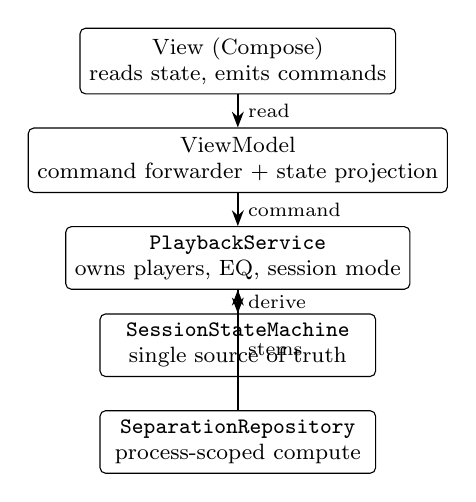
\begin{tikzpicture}[
    box/.style={draw, rounded corners=2pt, align=center, font=\footnotesize,
                minimum width=3.5cm, minimum height=0.75cm},
    layer/.style={draw, dashed, rounded corners=3pt, inner sep=4pt},
    arr/.style={-{Stealth[length=2mm]}, thick}
]
\node[box] (view) {View (Compose)\\ reads state, emits commands};
\node[box, below=0.42cm of view] (vm) {ViewModel\\ command forwarder + state projection};
\node[box, below=0.42cm of vm] (svc) {\texttt{PlaybackService}\\ owns players, EQ, session mode};
\node[box, below=0.30cm of svc] (sm) {\texttt{SessionStateMachine}\\ single source of truth};
\node[box, below=0.42cm of sm] (repo) {\texttt{SeparationRepository}\\ process-scoped compute};
\draw[arr] (view) -- node[right, font=\scriptsize]{read} (vm);
\draw[arr] (vm) -- node[right, font=\scriptsize]{command} (svc);
\draw[arr] (svc) -- node[right, font=\scriptsize]{derive} (sm);
\draw[arr] (repo) -- node[right, font=\scriptsize]{stems} (svc);
\end{tikzpicture}
\caption{Layer boundaries are drawn by \emph{ownership}, not by the
MVC/MVP/MVVM triad. The ViewModel no longer owns state; the service does, and
the state machine inside it is the single source of truth.}
\label{fig:arch}
\end{figure}

\subsection{Invariants as Design Rules}

Rather than validating state after the fact, we encode four invariants so that
illegal states cannot be constructed: (I1) a single-track item must belong to
the current queue, enforced at the queue-set entry point; (I2) equaliser
availability is a \emph{derived} property, not a stored flag; (I3) a separation
task transitions once, and only a genuine transition triggers the automatic
switch to multi-track; (I4) the playing state has one source. The governing
principle is: \emph{derive what can be derived; make invalid states
unrepresentable rather than repaired}.

Table~\ref{tab:sm} states the transitions explicitly. Each row is a small,
testable unit: the invariants become assertions on the transition function
rather than comments scattered through the UI.

\begin{table}[t]
\begingroup
\centering
\footnotesize
\nohyph
\setlength{\tabcolsep}{3pt}
\begin{tabular}{@{}l l l@{}}
\hline
\textbf{From} & \textbf{Event} & \textbf{To} \\
\hline
Idle        & load(track)        & Single \\
Single      & load(track)        & Single (queue replaced) \\
Single      & separate(start)    & Separating \\
Separating  & progress           & Separating \\
Separating  & done               & Multi (auto switch) \\
Separating  & cancel             & Single \\
Multi       & exit               & Single \\
Multi       & load(track)        & Single (I1: exit first) \\
\hline
\end{tabular}
\caption{Session transitions. Illegal transitions (for example moving to
multi-track without a completed separation) are absent by construction, which
is what invariant I3 enforces.}
\label{tab:sm}
\endgroup
\end{table}

\subsection{The Separation Pipeline: Satisfying N2}\label{sec:pipeline}

The pipeline is the part that interacts most directly with N2. Chunking is not
an optimisation here; it is the only way the requirement can be met.
Figure~\ref{fig:pipe} shows why it must be chunked: a whole-track spectrogram
does not fit, whereas a bounded chunk plus a cross-fade between consecutive
chunks does. The overlap exists because each inference call loses up to one
analysis hop at its boundaries; blending the tail of one chunk with the head of
the next hides this.

\begin{figure}[t]
\centering
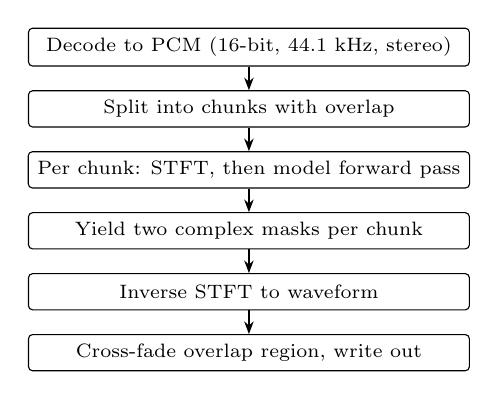
\begin{tikzpicture}[node distance=0.30cm,
    blk/.style={draw, rounded corners=1.5pt, font=\scriptsize, align=center,
                minimum width=5.6cm, minimum height=0.46cm},
    arr/.style={-{Stealth[length=1.6mm]}, semithick}]
\node[blk] (in)  {Decode to PCM (16-bit, 44.1 kHz, stereo)};
\node[blk, below=of in] (ch)  {Split into chunks with overlap};
\node[blk, below=of ch] (stft){Per chunk: STFT, then model forward pass};
\node[blk, below=of stft] (sep){Yield two complex masks per chunk};
\node[blk, below=of sep] (istft){Inverse STFT to waveform};
\node[blk, below=of istft] (mix){Cross-fade overlap region, write out};
\foreach \a/\b in {in/ch, ch/stft, stft/sep, sep/istft, istft/mix}
  \draw[arr] (\a) -- (\b);
\end{tikzpicture}
\caption{Offline separation pipeline. Chunking bounds memory (N2); the overlap
and cross-fade remove boundary artefacts introduced by per-chunk inference.}
\label{fig:pipe}
\end{figure}

\subsection{Concurrency Model: Satisfying N4}

Three kinds of work must not block one another: decoding, inference, and
rendering. Decoding and inference run on a background dispatcher owned by the
separation repository, which is process-scoped so that a job survives the
screen closing. Rendering is owned by ExoPlayer on its own internal threads;
the ViewModel never touches it directly. A small notification message passes
state from the compute side back to the service, and the service publishes it
as session state.

This separation matters for two reasons. It keeps the UI thread free during a
thirty-second separation, preserving responsiveness; and it means a
separation that outlives the activity is still observable when the user
returns, which is the practical form of requirement N5.

\subsection{Deliberate Deviations}

We use media3's custom-command channel to reach the service across the process
boundary. This means multi-track control does not flow through a single
reducer, and therefore the architecture is not MVI. We accept this: collapsing
everything into one reducer would require routing background playback through
a channel that does not survive the activity, trading architectural purity for
a broken N4 requirement.

\subsection{Design Trade-offs}

The choices below are the ones we expect to be questioned. Each is a place
where a simpler design exists and was rejected for a stated reason; being
explicit about them is what makes the architecture defensible rather than
merely different. They are given as a list rather than a table because each
entry carries a full-sentence justification, which a narrow column renders
unreadable.

\begin{description}
\item[Service-owned state.] \emph{Instead of} keeping state in the ViewModel:
  a ViewModel is destroyed with its host, so playback and separation would be
  interrupted exactly when they must persist.

\item[Multi-instance playback.] \emph{Instead of} one player mixing in PCM:
  mixing in the audio graph would mean implementing a mixer and re-deriving
  tempo and pitch ourselves, duplicating work the platform already does.

\item[Streaming data source.] \emph{Instead of} writing stems to files first:
  a file is only playable once its header is final, which is precisely what
  defeats playback before separation finishes.

\item[Shared audio focus.] \emph{Instead of} one focus request per track: only
  one instance can hold focus, and the system would pause the others.

\item[Staged model tiers.] \emph{Instead of} one model for all devices: a
  single model is either too slow on weak hardware or too poor on strong
  hardware.
\end{description}

\subsection{Walkthrough of a Typical Session}

A walkthrough makes the design concrete. A learner opens the application and
sees the player screen. They import a track; the player enters the single
state and the waveform is extracted. They drag the waveform to the first verse
and press play. They then switch to the separation screen and choose the two
stem fast tier. The service begins separating from the current playback
position rather than from the beginning, which is the difference between
waiting seconds and waiting minutes.

When the first segment is ready, the player switches to multi-track and resumes
at the position it left. The learner drags the vocal track to zero and hears
the accompaniment alone. They slow the tempo to practise a passage; both stems
follow because tempo is applied to the session rather than to one player. On
finishing, they exit multi-track and the original track resumes, with the
stems still cached for later.

Every transition in this walkthrough corresponds to a row in
Table~\ref{tab:sm}. That correspondence is the point: the interaction model and
the state machine are the same object viewed from two angles.

\subsection{Privacy and Data Handling}

The application requests no network permission for its core path. Audio never
leaves the device; there is no account and no telemetry. This is a
direct consequence of the Humanitarian positioning: a learner using the tool
on a borrowed or shared phone does not create a remote record of what they are
studying. Model files are the only downloads, and they are handled by an
explicit user action rather than automatic background fetching.

\section{Implementation Status}

A de-risking spike was carried out before writing this proposal, following the
practice of validating the highest-risk assumptions first. It established three
things on a mid-range device (MediaTek Helio G100, 12~GB):

\begin{itemize}
\item Fully offline two-stem separation runs at approximately 7.9x real time,
so a four-minute track separates in about thirty seconds.
\item Chunked streaming separation produces sample-aligned stereo stems without
exhausting the heap at a thirty-second chunk size.
\item A multi-track ExoPlayer session can be driven from a foreground service,
satisfying background playback and the media-notification requirement.
\end{itemize}

The spike covers the highest-risk portion of the workload---the inference
pipeline and the multi-track playback core---and is what makes the remaining
design credible. Figure~\ref{fig:ui} shows four screens from the spike.

\paragraph{Model selection.} Three families of open model were considered.
Their measured behaviour on the target device differs by an order of magnitude,
which is what makes tiering necessary rather than decorative.

\begin{table}[t]
\begingroup
\centering
\footnotesize
\nohyph
\setlength{\tabcolsep}{3pt}
\begin{tabular}{@{}l r r l@{}}
\hline
\textbf{Model} & \textbf{Speed} & \textbf{Memory} & \textbf{Role} \\
\hline
Spleeter 2-stem & $\approx$8$\times$ & $\approx$0.7\,GB & default, always available \\
Spleeter 4-stem & $\approx$3$\times$ & $\approx$1.2\,GB & optional quality tier \\
UVR (small)     & $\approx$1$\times$ & $\approx$1.1\,GB & optional, slow tier \\
UVR (large)     & $\approx$0.3$\times$ & $\approx$2.0\,GB & high quality, rarely real time \\
Demucs          & $\approx$0.6$\times$ & very high   & research only \\
\hline
\end{tabular}
\caption{Measured relative speed (times real time) and memory on a mid-range
device. A model that runs below $1\times$ cannot be used in a position-from-playback
workflow, which is why such models are offered only as an explicit
``separate first, then listen'' path.}
\label{tab:models}
\endgroup
\end{table}

The consequence for the design is direct. A single model cannot serve both a
cheap phone and an expensive one: the fast model wastes the expensive phone's
capability, and the slow model makes the cheap phone unusable. The benchmark
layer exists to choose between them at run time, and the tier grouping is what
the user actually sees.

\begin{figure}[t]
\centering
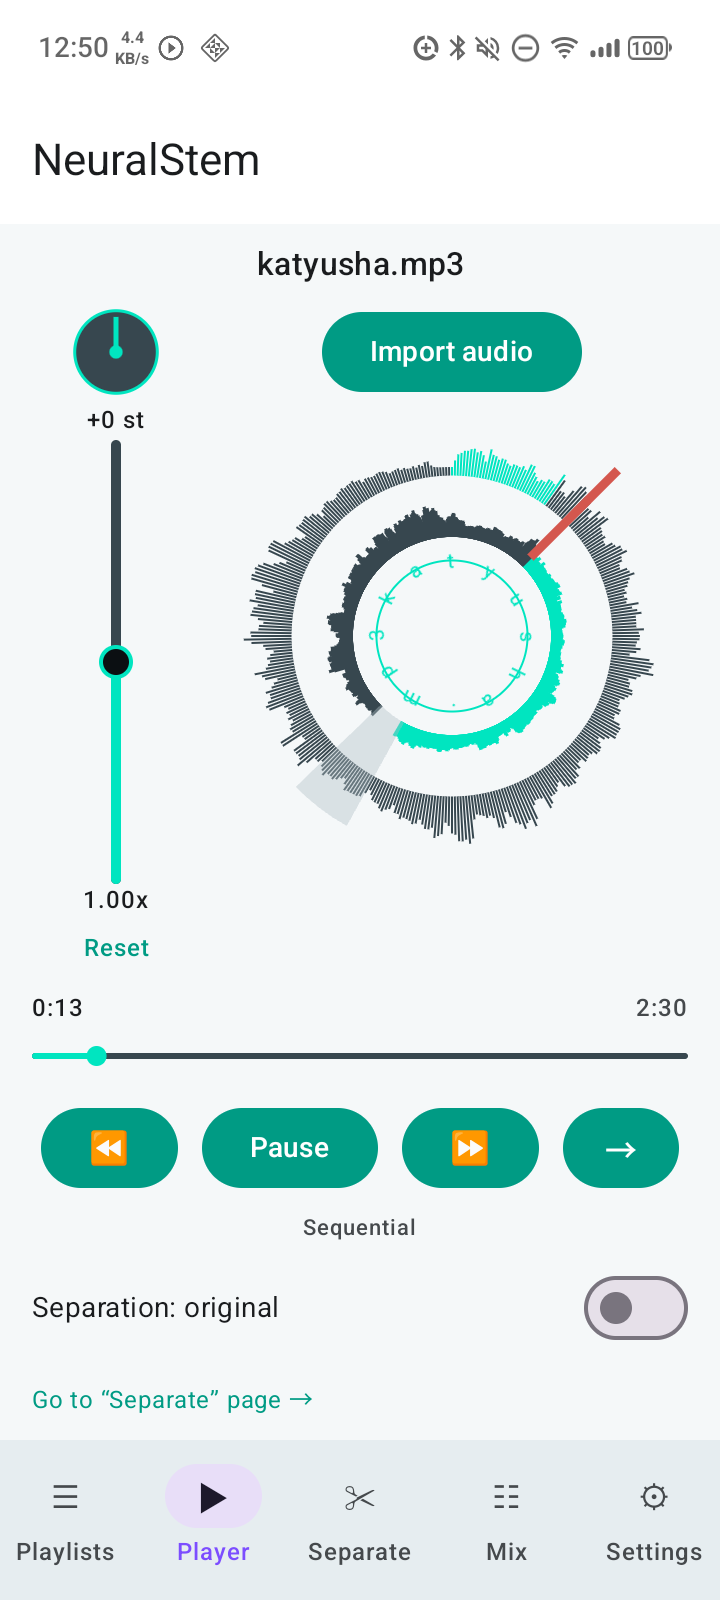
\includegraphics[width=0.23\columnwidth]{figures/1_player.png}\hfill
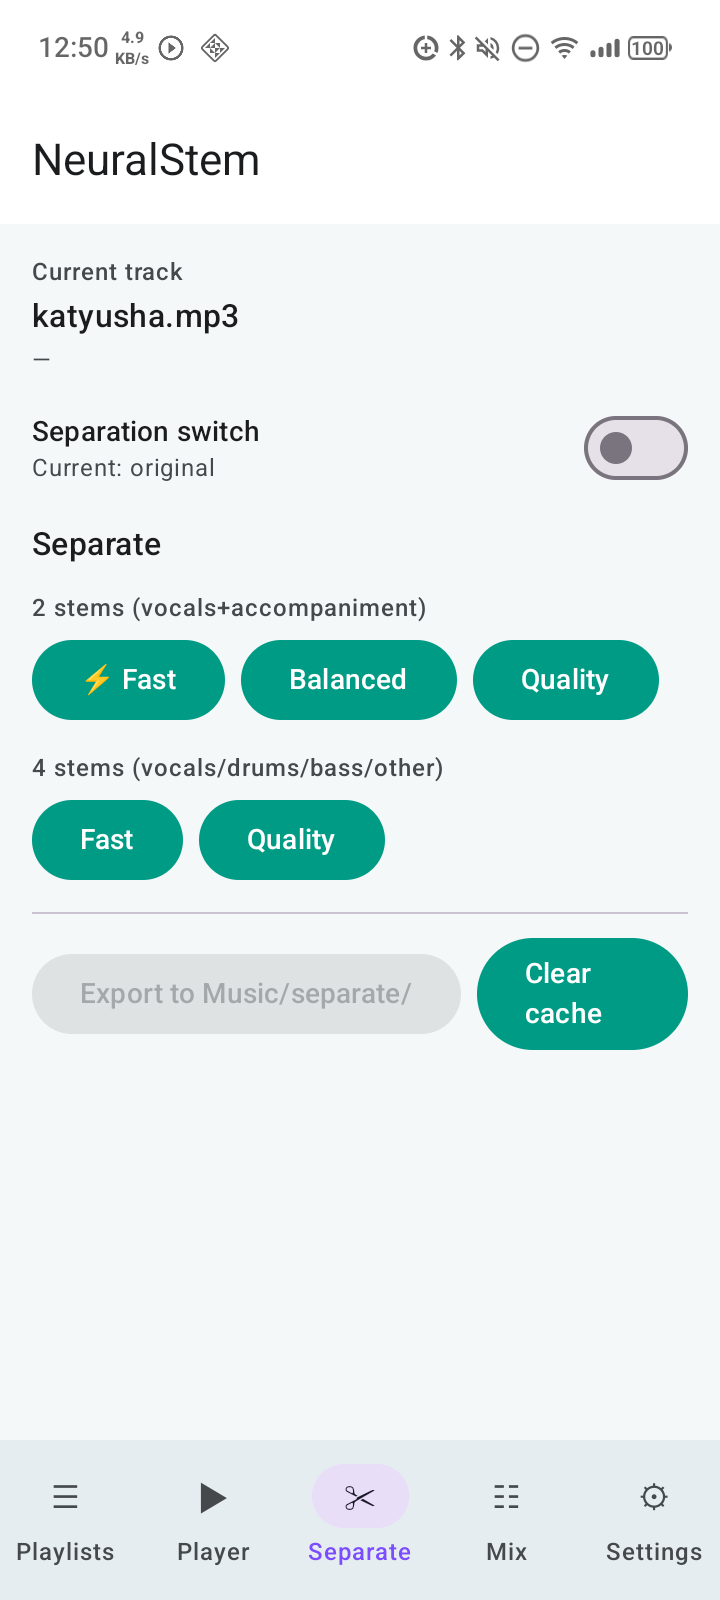
\includegraphics[width=0.23\columnwidth]{figures/2_separate.png}\hfill
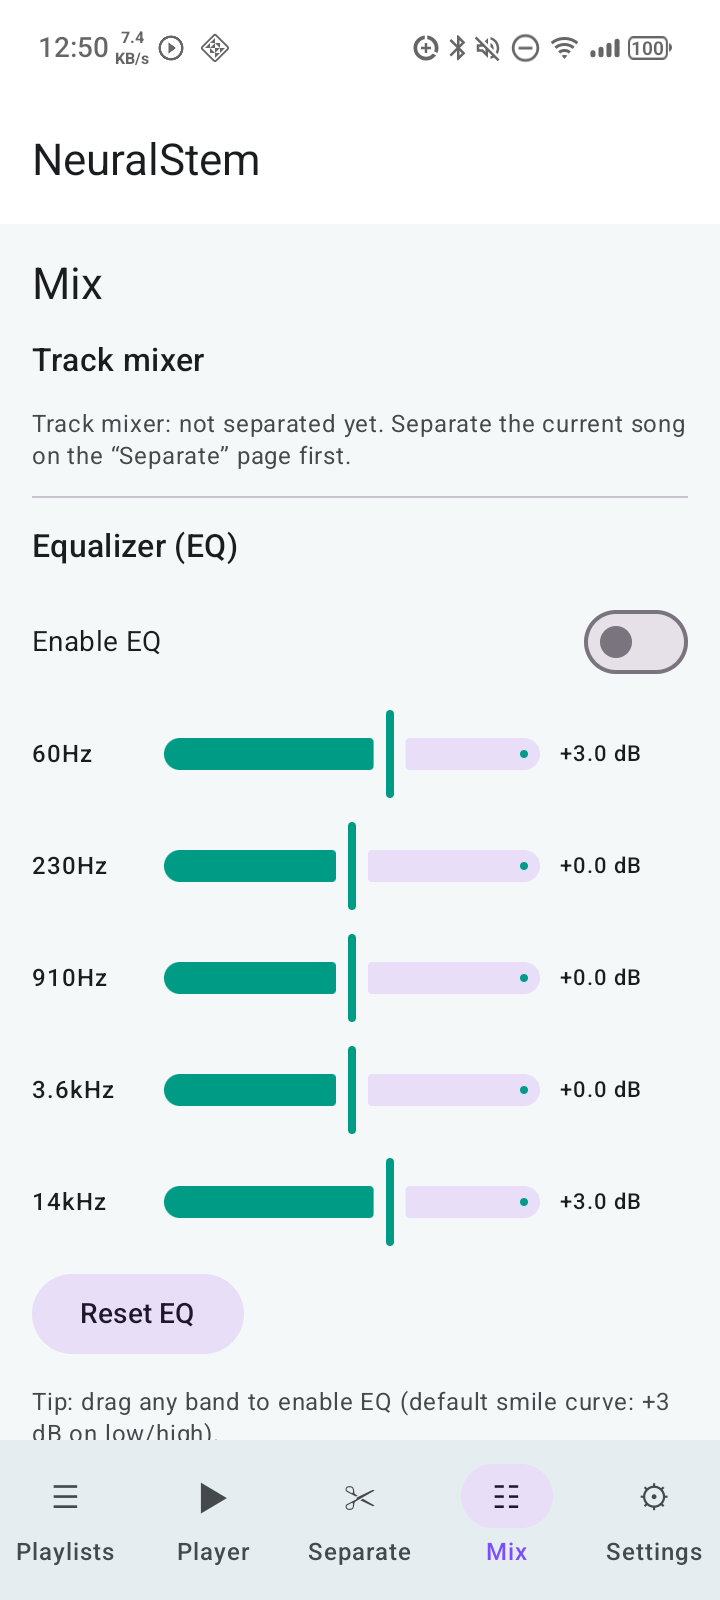
\includegraphics[width=0.23\columnwidth]{figures/3_mix.png}\hfill
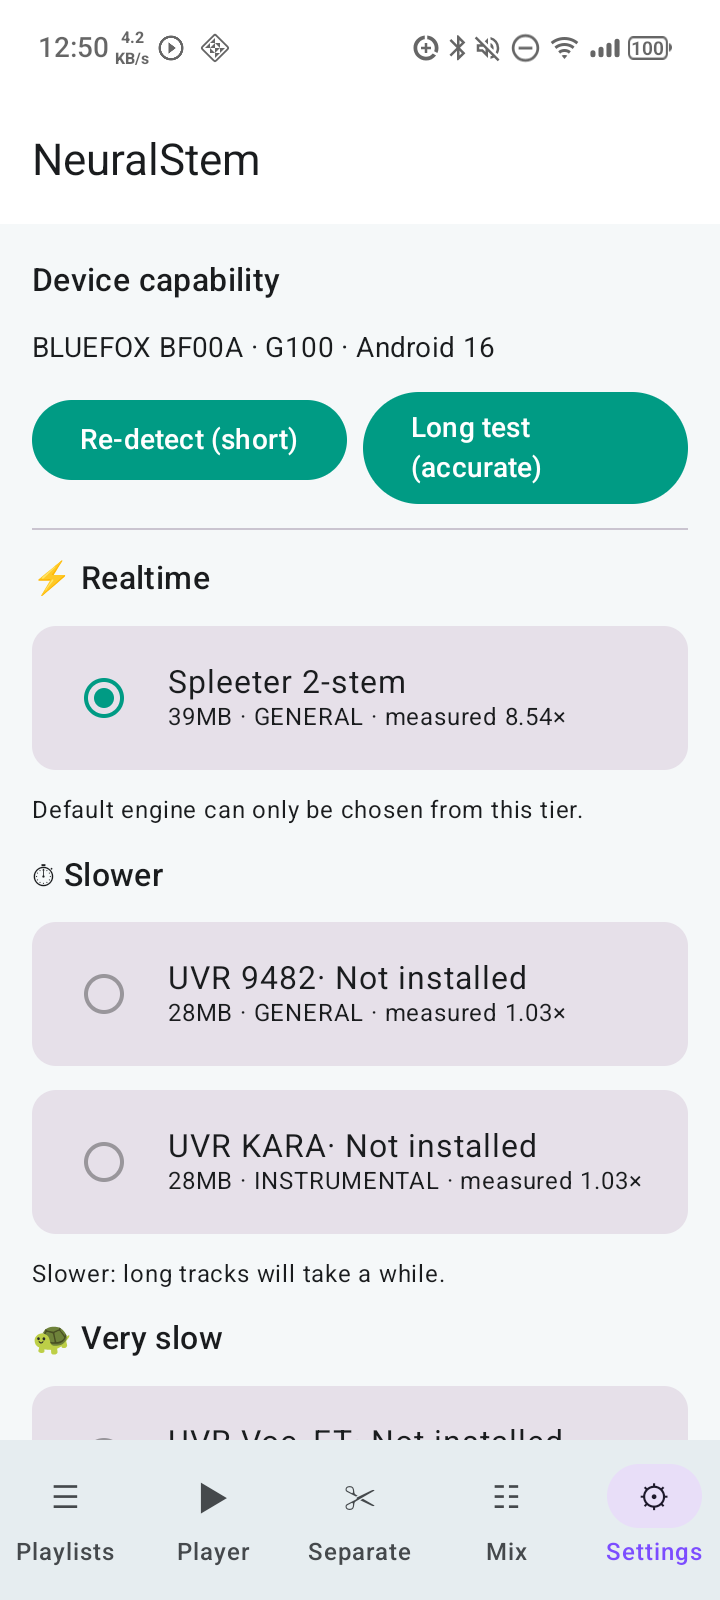
\includegraphics[width=0.23\columnwidth]{figures/4_settings.png}
\caption{Spike screens, left to right: player (turntable, waveform, tempo and
pitch); separation (tier selection by number of stems); mix (per-track gain,
mute, solo and equaliser); settings (device capability and model tiers).}
\label{fig:ui}
\end{figure}

\section{Feasibility and Scope}

The concern with a project of this ambition is that it cannot be finished by
one student. We address this directly.

\paragraph{The spike proves the hard part.} The expensive unknowns are model
inference on a phone and synchronised multi-track rendering; both are
demonstrated. What remains is application work on a known foundation:
playlists, export, model download, and interface polish.

\paragraph{Scope is deliberately staged.} Two-stem separation is the shipping
feature; four-stem and larger models are optional tiers selected by the device
benchmark. This means the app is \emph{useful} at the end of the core
milestone, and subsequent models are additive rather than prerequisites.

\paragraph{The workload is measured, not asserted.} The spike includes unit
tests for the separator geometry and the multi-track alignment, so the
foundation is verifiable rather than merely demonstrated by hand.

\paragraph{What remains, and what could go wrong.} Five risks are still open.
Each has a concrete mitigation and, importantly, a fallback that preserves a
shippable application.

\begin{description}
\item[Slow phones cannot run large models] The impact is a quality ceiling.
  Benchmark tiers keep the fast two-stem model as the guaranteed baseline.

\item[Memory pressure with four stems] The impact is a crash on low-RAM
  devices. Models are kept outside the Java heap, and four stems are offered
  only where the benchmark permits.

\item[State machine misses a transition] The impact is an inconsistent
  interface, prevented by invariants I1--I4 and unit tests on the transition
  table.

\item[Model licence restrictions] The impact is a licence conflict. Licences
  are shown per model, and weights are downloaded from the origin rather than
  bundled.

\item[Scope overrun] The impact is an unfinished project. The core milestone
  is the two-stem path and everything else is additive, so the project remains
  useful even if no optional tier is reached.
\end{description}

\section{Development Method}

The spike was not written as a demonstration but as an instrument. Three
practices shaped it and will continue into the remaining milestones.

\paragraph{Test the invariants, not the screens.} Most automated tests exercise
pure logic: the transition table, the chunk geometry, the resampler, and the
alignment of two stems after a seek. Interface behaviour is verified separately
and more coarsely. The reason is that the defects which cost the most time in
the spike were state inconsistencies rather than broken views, and state logic
is cheap to test exhaustively.

\paragraph{Verify through channels that do not lie.} A test that clicks at a
screen coordinate breaks whenever a layout moves, and a log line proves only
that a log line was written. The spike therefore checks behaviour through the
system rather than through the pixels: whether the audio subsystem reports the
expected number of active tracks, whether a cache file exists with the right
size, whether the playback position actually advanced.

\paragraph{Keep the risky path short.} The two-stem fast path was built and
verified first. Everything that adds risk---larger models, four stems, a
benchmark layer---was added only after the core could be demonstrated end to
end. This is the same ordering used to justify the staged scope above.

\section{Evaluation Plan}

Evaluation will not be a single-device speed contest. We will assess three
questions. First, \emph{does separation succeed on the target device class}
within a time budget a learner tolerates? Second, \emph{is the multi-track
experience correct}---do stems remain aligned after seeking and tempo changes,
and does per-track gain behave as expected? Third, \emph{is the interaction
discoverable}---can a first-time user separate a track and isolate a part
without instruction? The first two are instrumented; the third requires a small
number of users.

Table~\ref{tab:mile} gives the remaining milestones. They are ordered so that
the application is demonstrable after every step rather than only at the end.

\begin{table}[t]
\begingroup
\centering
\footnotesize
\nohyph
\setlength{\tabcolsep}{3pt}
\begin{tabular}{@{}l >{\raggedright\arraybackslash}p{4.9cm}@{}}
\hline
\textbf{Milestone} & \textbf{Content} \\
\hline
M1 & Close the two-stem path: import, separate, play stems with per-track
     gain and solo. \\
M2 & Temperament and equaliser polish; persist session state across restarts. \\
M3 & Four-stem tier, gated by the device benchmark. \\
M4 & Model manager: download on demand, verify integrity, show per-model
     licence. \\
M5 & Playlist and export; final evaluation and write-up. \\
\hline
\end{tabular}
\caption{Remaining milestones. M1 alone yields a usable application, which is
what makes the staged scope safe.}
\label{tab:mile}
\endgroup
\end{table}

\section{Quality Assurance: Limitations and Threats to Validity}

This section collects everything that constrains the claims above, so that the
reader can judge them together rather than piecemeal.

\subsection{Product Limitations}

The separation quality is bounded by the open models: the two-stem Spleeter
model was trained in 2019 and leaks and dulls high frequencies. Larger models
separate better but are substantially slower on mid-range hardware. Streaming
separation is currently offered only for the fastest tier. Model weights carry
their own licences, which differ---in particular, some vocal-remover weights
are restricted to non-commercial use; the app must present these per model
rather than under a single licence.

\subsection{Threats to Validity}

We are deliberate about what the spike does and does not establish, because a
single successful demonstration can be over-read.

\paragraph{External validity.} All measurements were taken on one mid-range
device with a MediaTek Helio G100 and 12~GB of memory. Absolute speeds will
not transfer to other hardware, and we therefore report them as evidence that
the pipeline runs at usable speed, not as a ranking of models. The tiering
layer exists precisely because the absolute numbers are device-dependent;
the right response to a different device is to re-measure, which the
application does on first launch rather than relying on a table shipped in the
source.

\paragraph{Construct validity.} Speed is measured as the ratio of audio
duration to inference time. This is the metric a learner feels, but it ignores
first-segment latency, which is what determines how long the user waits before
hearing anything. We report it separately in the interface rather than folding
it into a single figure.

\paragraph{Quality is not established by these measurements.} That a separator
runs quickly says nothing about how well it separates. Objective spectral
measures correlate only loosely with what a listener judges to be usable for
practice, so the quality claim in this proposal is deliberately weak: the
models are the best openly available, and the acceptance question is whether a
learner finds the result useful, which requires listening rather than
automated scoring.

\paragraph{Small-scale user evidence.} The interaction claims rest on design
reasoning rather than on a controlled study. This is appropriate for a proposal
but is a limitation of any claim about discoverability, and the evaluation plan
treats it as such.

\subsection{Why the Core Deliverable Still Holds}

Taken together these threats limit how strongly the results can be claimed, but
they do not endanger the deliverable. Each is bounded by a mitigation already
described: device dependence is handled by measuring on the user's own hardware
rather than trusting a table; quality expectations are set by presenting the
model tier honestly rather than promising studio results; and the staged scope
means that a weaker-than-hoped model still yields a working practice tool. The
risk that remains---that the models are simply not good enough to be
useful---is the one risk no engineering decision can remove, and it is the
reason the evaluation plan asks real learners rather than relying on a metric.

\section{Reproducibility}

The implementation is public and builds from source. The repository contains the
Android project, the native glue for the inference runtime, and the automated
tests; model weights are deliberately excluded because of their size and
because their licences differ, and are obtained by the user. A continuous
integration job builds the application and runs the test suite on every push,
so that the state of the project is observable rather than asserted.

This matters for assessment as well as for engineering. A reader can check any
claim in this proposal against the code and its test results, rather than
taking them on trust.

\section{Conclusion}

NeuralStem turns an existing research capability into a tool that a learner can
use on the phone they already own, with no network and no subscription. The
architecture---MVVM in its layers, but with a service-owned Model and a
state-machine core---follows from the lifetime and combinatorial properties of
the problem rather than from convention, and a de-risking spike has shown that
the two hardest parts already work.

\section*{AI Use Statement}
AI assistants were used for routine coding support and for editorial help in
preparing this document. All architectural decisions, scope choices and
technical claims were reviewed and can be defended by the author.

\begin{thebibliography}{99}

\bibitem[Hennequin et~al.(2020)Hennequin, Khlif, and Voituret]{hennequin2020spleeter}
Romain Hennequin, Anis Khlif, and F\'elix Voituret.
\newblock Spleeter: A fast and efficient music source separation tool with
  pre-trained models.
\newblock {\em Journal of Open Source Software}, 5(50):2154, 2020.

\bibitem[Rouard et~al.(2023)Rouard, Massa, and D\'efossez]{rouard2023demucs}
Simon Rouard, Francisco Massa, and Alexandre D\'efossez.
\newblock Hybrid transformers for music source separation.
\newblock In {\em Proceedings of the IEEE International Conference on Acoustics,
  Speech and Signal Processing (ICASSP)}, 2023.

\bibitem[{ONNX Runtime}(2025)]{onnxruntime}
Microsoft.
\newblock ONNX Runtime: Cross-platform, high performance scoring engine for
  machine learning models.
\newblock \url{https://github.com/microsoft/onnxruntime}, 2025.
\newblock Accessed 2026.

\bibitem[{sherpa-onnx}(2025)]{sherpaonnx}
k2-fsa.
\newblock sherpa-onnx: Speech recognition, text-to-speech and source separation
  without internet connection.
\newblock \url{https://github.com/k2-fsa/sherpa-onnx}, 2025.
\newblock Accessed 2026.

\bibitem[{Android Developers}(2025)]{media3}
Android Developers.
\newblock Media3 ExoPlayer and MediaSessionService.
\newblock \url{https://developer.android.com/media/media3}, 2025.
\newblock Accessed 2026.

\bibitem[{Android Developers}(2025b)]{androidstorage}
Android Developers.
\newblock Storage Access Framework and document providers.
\newblock \url{https://developer.android.com/guide/topics/providers/document-provider},
  2025.
\newblock Accessed 2026.

\bibitem[{Android Developers}(2025c)]{androidfg}
Android Developers.
\newblock Foreground services and notifications.
\newblock
  \url{https://developer.android.com/develop/background-work/services/fgs}, 2025.
\newblock Accessed 2026.

\end{thebibliography}

\end{document}
